\documentclass{article}
\usepackage{pdfpages}
\usepackage{graphicx}  % For PNG
\usepackage[left=2cm, right=2cm, top=2cm]{geometry}
\usepackage[newfloat]{minted}
\usepackage{enumitem}
% Give Table of Contents Hyperlinks
\usepackage{hyperref}
\hypersetup{
    colorlinks,
    citecolor=black,
    filecolor=black,
    linkcolor=black,
    urlcolor=blue
}
% \renewcommand{\theenumi}{\Alph{enumi}} % https://tex.stackexchange.com/a/2292

\pagenumbering{gobble}
% \pagenumbering{roman} % set the numbering style to lowercase letter

\title{\textbf{Homework 5}}

\author{MacMillan, Kyle}
\date{November 26, 2018}

\begin{document}


\addcontentsline{toc}{section}{Title}
\maketitle

\newpage
\tableofcontents
\addcontentsline{toc}{section}{Table of Contents}
\newpage
\listoffigures
\addcontentsline{toc}{section}{List of Figures}

\pagenumbering{roman}   % Set TOC page numbering to lowercase roman numerals


%%%%%%%%%%%%%%%%%%%%%%%%%%%% INTRO SECTION %%%%%%%%%%%%%%%%%%%%%%%%%%%%
\newpage
\hypersetup{
    colorlinks,
    citecolor=blue,
    filecolor=black,
    linkcolor=blue,
    urlcolor=blue
}
\pagenumbering{arabic}  % Set content page numbering to arabic numerals

\setcounter{page}{1}
\newpage
\section{\textbf{Chapter 11}}
\subsection{Problem 3}
To accomplish this problem I created a class to generate a random map of any 
size you want up to 99. It generates a random number of obstacles of random 
size. Play around with it, it's fun. You can change the random numbers or just 
run the file multiple times. Code for this problem can be found 
\href{https://github.com/macattackftw/RoboticsHW/blob/master/HW5/problem11_3.py}{here}.

Demonstration is shown in Figure \ref{fig:p11_3_1}. This is an application of 
the WaveFront BFS algorithm. From there it goes on to find the shortest path as 
seen in Figure \ref{fig:p11_3_2}.

The seed for that particular example is: \texttt{7635686187880284248}

\begin{figure}[h]
    \centering
    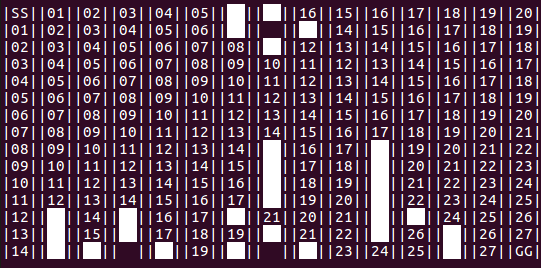
\includegraphics[scale=2.5]{problem11_3_1}
    \caption{WaveFront Distance Evaluation}
    \label{fig:p11_3_1}
\end{figure}

\begin{figure}[h]
    \centering
    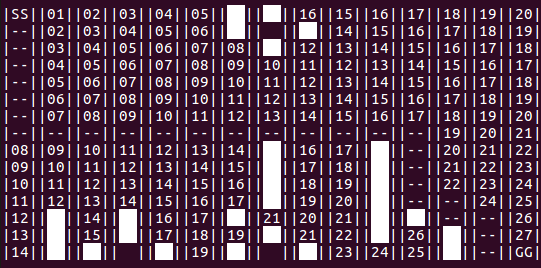
\includegraphics[scale=2.5]{problem11_3_2}
    \caption{WaveFront Shortest Path}
    \label{fig:p11_3_2}
\end{figure}

The book constantly refers to this as a start to goal process but that is not 
how flood-fill works because you can not guarantee shortest path; you can not 
have it both ways. The book calls for ``minimal path'' but then uses a 
non-optimal solver. I wrote it as the book asked the first time around then 
changed it to actually give the optimal answer because that's what we want.

To clarify: Starting from the start is fine but you have to traverse it 
backwards from goal to start. The reason is because you do not know which of the 
``equal'' numbers to choose when you're walking from start to goal. You 
\textbf{know} which path is the shortest if you walk from goal to start. If two 
numbers are the same then either path is optimal/minimal.

\newpage
\section{\textbf{Chapter 16}}
\subsection{Problem 1}
asdf

\subsection{Problem 2}
Given 40 measurements at 2 meters we can subtract the 2 meters and then take 
the mean:

\begin{enumerate}[label=\Alph*]
    \item 0.23521735
    \item -0.13556097
    \item 0.33806001
\end{enumerate}

That is how far off each senor averages from 2 meters. Each new sensor reading 
then has that mean subtracted from it to yield:

\begin{enumerate}[label=\Alph*]
    \item 2.22255225
    \item 2.03233526
    \item 1.79719609
\end{enumerate}

We can then take the mean of those values for an expected distance of: 
\texttt{2.0173612016666667}. The code for this can be found 
\href{}{here} 
and in the code snippet \ref{code:16_2}.

\begin{code}
\label{code:16_2}
\begin{minted}{python}
    dist_sens -= 2
    mean = np.mean(dist_sens, dtype=np.float64, axis=0)
    new_sens = np.array([[2.4577696, 1.8967743, 2.1352561]]) - mean
    distance = np.mean(new_sens)
\end{minted}
\end{code}


\newpage
\section{\textbf{Chapter 17}}
\subsection{Problem 2}
asdf


\subsection{Problem 3}
asdf


\subsection{Problem 4}
asdf



\newpage
\section{\textbf{Chapter 18}}
\subsection{Problem 1}
\subsubsection{Problem 1.1}
asdf


\subsubsection{Problem 1.2}
asdf


\subsubsection{Problem 1.3}
asdf


\end{document}
